\documentclass[border=2pt]{standalone}
\usepackage{tikz}
\usetikzlibrary{petri}
    \tikzset{>=latex}
\usepackage{diffcoeff}

\begin{document}
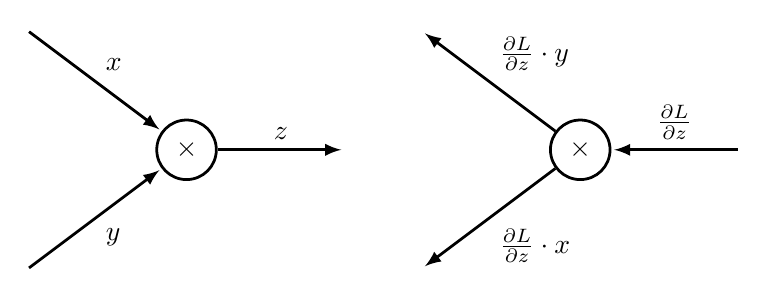
\begin{tikzpicture}[line width=1pt]
    \coordinate (fpx) at (-2, 1.5);
    \coordinate (fpy) at (-2, -1.5);
    \coordinate (fpz) at (2, 0);

    \node[place] at (0, 0) {$ \times $}
    edge [pre] node[above right] {$ x $} (fpx)
    edge [pre] node[below right] {$ y $} (fpy)
    edge [post] node[above] {$ z $} (fpz);

    \coordinate (bpx) at (3, 1.5);
    \coordinate (bpy) at (3, -1.5);
    \coordinate (bpz) at (7, 0);
    \node[place] at (5, 0) {$ \times $}
    edge [post] node[above right] {$ \diffp{L}{z} \cdot y $} (bpx)
    edge [post] node[below right] {$ \diffp{L}{z} \cdot x $} (bpy)
    edge [pre] node[above] {$ \diffp{L}{z} $} (bpz);
\end{tikzpicture}
\end{document}